\documentclass[a4paper]{article} 
\addtolength{\hoffset}{-2.25cm}
\addtolength{\textwidth}{4.5cm}
\addtolength{\voffset}{-3.25cm}
\addtolength{\textheight}{5cm}
\setlength{\parskip}{0pt}
\setlength{\parindent}{0in}

%----------------------------------------------------------------------------------------
%	PACKAGES AND OTHER DOCUMENT CONFIGURATIONS
%----------------------------------------------------------------------------------------

\usepackage[italicdiff]{physics}
%\usepackage{derivative}
\usepackage{tasks}
\usepackage{blindtext} % Package to generate dummy text
\usepackage{charter} % Use the Charter font
\usepackage[utf8]{inputenc} % Use UTF-8 encoding
\usepackage{microtype} % Slightly tweak font spacing for aesthetics
\usepackage[T1]{fontenc}
\usepackage{polski}
\usepackage{enumerate}
\usepackage[utf8]{inputenc}
\usepackage[english, ngerman]{babel} % Language hyphenation and typographical rules
\usepackage{amsthm, amsmath, amssymb} % Mathematical typesetting
\usepackage{float} % Improved interface for floating objects
\usepackage[final, colorlinks = true, 
            linkcolor = black, 
            citecolor = black]{hyperref} % For hyperlinks in the PDF
\usepackage{graphicx, multicol} % Enhanced support for graphics
\usepackage{xcolor} % Driver-independent color extensions
\usepackage{marvosym, wasysym} % More symbols
\usepackage{rotating} % Rotation tools
\usepackage{censor} % Facilities for controlling restricted text
\usepackage{listings, style/lstlisting} % Environment for non-formatted code, !uses style file!
\usepackage{pseudocode} % Environment for specifying algorithms in a natural way
\usepackage{style/avm} % Environment for f-structures, !uses style file!
\usepackage{booktabs} % Enhances quality of tables
\usepackage{tikz-qtree} % Easy tree drawing tool
\tikzset{every tree node/.style={align=center,anchor=north},
         level distance=2cm} % Configuration for q-trees
\usepackage{style/btree} % Configuration for b-trees and b+-trees, !uses style file!
\usepackage[backend=biber,style=numeric,
            sorting=nyt]{biblatex} % Complete reimplementation of bibliographic facilities
\addbibresource{ecl.bib}
\usepackage{csquotes} % Context sensitive quotation facilities
\usepackage[yyyymmdd]{datetime} % Uses YEAR-MONTH-DAY format for dates
\renewcommand{\dateseparator}{-} % Sets dateseparator to '-'
\usepackage{fancyhdr} % Headers and footers
\pagestyle{fancy} % All pages have headers and footers
\fancyhead{}\renewcommand{\headrulewidth}{0pt} % Blank out the default header
\fancyfoot[L]{} % Custom footer text
\fancyfoot[C]{} % Custom footer text
\fancyfoot[R]{\thepage} % Custom footer text
\newcommand{\note}[1]{\marginpar{\scriptsize \textcolor{red}{#1}}} %
\graphicspath{ {./images/} }

%----------------------------------------------------------------------------------------

\begin{document}

%-------------------------------
%	TITLE SECTION
%-------------------------------

\fancyhead[C]{}
\hrule \medskip % Upper rule
\begin{minipage}{0.295\textwidth} 
\raggedright
\footnotesize
Antoni Dąbrowski \hfill\\   
Nr. indeksu 317214\hfill\\
Mail: 317214@uwr.edu.pl
\end{minipage}
\begin{minipage}{0.4\textwidth} 
\centering 
\large 
Statystyka\\ 
\normalsize 
Laboratorium - lista IV\\ 
\end{minipage}
\begin{minipage}{0.295\textwidth} 
\raggedleft
\today\hfill\\
\end{minipage}
\medskip\hrule 
\bigskip

%-------------------------------
%	CONTENTS
%-------------------------------


\section{Zadanie pierwsze}
Podaj przedział ufności dla różnicy dwóch średnich w modelu normalnym o znanych wariancjach na poziomie ufności $1-\alpha$. Uzasadnij jego postać.

\subsection{Rozwiązanie}
Niech $X_1,...,X_{n_1}\sim N(\mu_1,\sigma_1)$ oraz $Y_1,...,Y_{n_2}\sim N(\mu_1,\sigma_1)$. Znamy $\sigma_1, \sigma_2$. Interesuje nas przedział ufności dla parametru $\mu_1-\mu_2$. Jego estymatorem punktowym jest $\bar{X}-\bar{Y}$, gdzie $\bar{X}=\frac{1}{n_1}\sum_{i=1}^{n_1}X_i$ oraz $\bar{Y}=\frac{1}{n_2}\sum_{i=1}^{n_2}Y_i$

Przedziałem ufności na poziomie $1-\alpha$ szukanego parametru jest:
$$[(\bar{X}-\bar{Y})-z_{1-\alpha/2}\frac{\sigma}{\sqrt{n}},(\bar{X}-\bar{Y})+z_{1-\alpha/2}\frac{\sigma}{\sqrt{n}}],$$

gdzie $\sigma^2=\frac{\sigma_1^2}{n_1}+\frac{\sigma_2^2}{n_2}$
\section{Zadanie drugie}
Wygeneruj $n_1=50$ i $n_2=50$ obserwacji z rozkładu
\begin{enumerate}[a.]
	\item normalnego z parametrami przesunięcia $\mu_1$,$\mu_2$ i skali $\sigma_2$,$\sigma_2$
	\item logistycznego z parametrami przesunięcia $\mu_1$,$\mu_2$ i skali $\sigma_2$,$\sigma_2$
	\item Cauchy'ego z parametrami przesunięcia $\mu_1$,$\mu_2$ i skali $\sigma_2$,$\sigma_2$
\end{enumerate}

Na tej podstawie wyznacz przedziały ufności z zadania 1 dla parametru $\mu_1-\mu_2$ na poziomie ufności $1-\alpha=0.95$ oraz jego długość. Doświadczenie powtórz 10000 razy. Oszacuj prawdopodobieństwo pokrycia nieznanego parametru przez przedział ufności oraz jego długość. Przedyskutuj uzyskane wyniki.

\subsection{Rozwiązanie}
Poniższe wykresy przedstawiają $1\%$ spośród 10000 losowań 50-elementowych próbek. Zielona linia określa prawdziwą wartość estymowanego parametru. Pionowe słupki to przedziały ufności wokół estymatu punktowego, czerwone słupki oznaczają przedziały nie zawierające prawdziwej wartości. Pod wykresem podaję parametry rozkładu, liczbę błędnie określonych przedziałów ufności (takich, które nie pokrywają wartości rzeczywistej). Dalej podaję przedział ufności i jego długość wyznaczone jako mediana spośród wszystkich prób.

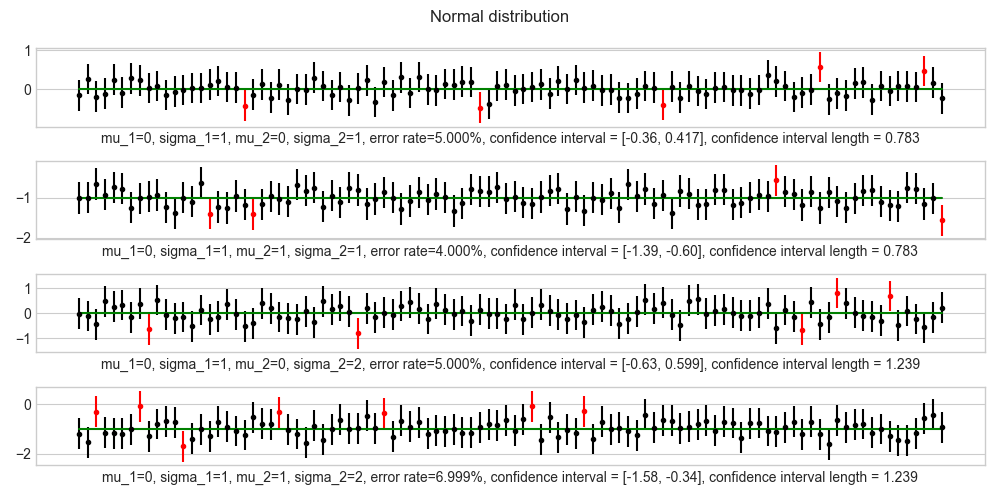
\includegraphics[scale=0.65]{Z2_a.png}

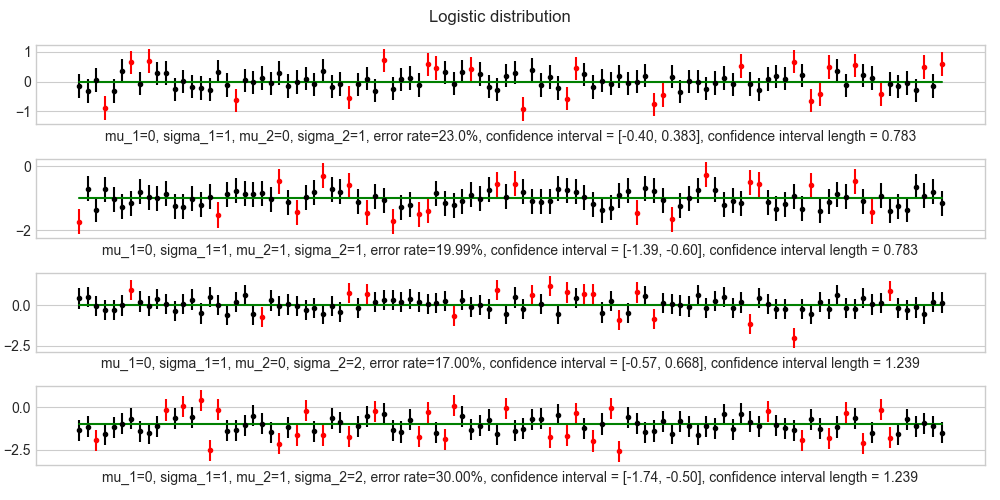
\includegraphics[scale=0.65]{Z2_b.png}

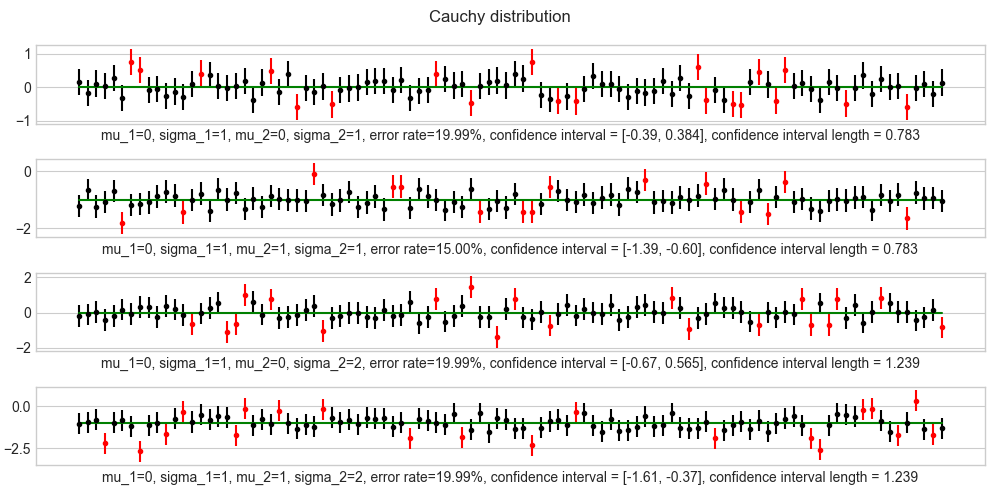
\includegraphics[scale=0.65]{Z2_c.png}

\textbf{Obserwacje:}

Teoria z zadania pierwszego sprawdza się w praktyce. Przedział ufności dla rozkładu normalnego i poziomu ufności $95\%$ faktycznie w takim stopniu pokrywa dokładną wartość. Nie jest tak jednak dla pozostałych rozkładów. Przyczynę tego spodziewam się znaleźć w nie dość dużej próbie, gdyż teoria mówi, że asymptotycznie powinniśmy otrzymać dobry przedział.

\section{Zadanie trzecie}
Podaj przedziały ufności dla różnicy dwóch średnich w modelu normalnym o nieznanych równych wariancjach na poziomie ufności $1-\alpha$. Uzasadnij jego postać.

\subsection{Rozwiązanie}
Tak jak w zadaniu piątym.

\section{Zadanie czwarte}
Powtórz eksperyment numeryczny z zadania 2 dla wybranych konfiguracji. Na jego podstawie oszacuj prawdopodobieństwo pokrycia nieznanego parametru przez przedział ufności z zadania 3 na poziomie ufności 0.95 oraz jego długość. Przedyskutuj uzyskane rezultaty.
\subsection{Rozwiązanie}
Tak jak w zadaniu szóstym.

\section{Zadanie piąte}
Podaj przedziały ufności dla różnicy dwóch średnich w modelu normalnym o nieznanych różnych wariancjach na poziomie ufności $1-\alpha$. Uzasadnij jego postać.

\subsection{Rozwiązanie}
Nie znane $\sigma_1, \sigma_2$.

Estymatory $\sigma_1, \sigma_2$, to $S_1^2=\frac{1}{n_1-1}\sum_{i=1}^{n_1}(X_i-\bar{X})^2$ i $S_2^2=\frac{1}{n_2-1}\sum_{i=1}^{n_2}(Y_i-\bar{Y})^2$.

Estymator $S_p=\frac{(n_1-1)S_1^2+(n_2-1)s_2^2}{n_1+n_2-2}$

Przedział ufności dla $\mu_1-\mu_2$ ma postać:
$$[(\bar{X}-\bar{Y})-t_{1-\alpha/2}(n_1+n_2-2)S_p\sqrt{\frac{1}{n_1}+\frac{1}{n_2}},(\bar{X}-\bar{Y})+t_{1-\alpha/2}(n_1+n_2-2)S_p\sqrt{\frac{1}{n_1}+\frac{1}{n_2}}]$$

\section{Zadanie szóste}
Powtórz eksperyment numeryczny z zadania 2 dla wybranych konfiguracji. Na jego podstawie oszacuj prawdopodobieństwo pokrycia nieznanego parametru przez przedział ufności z zadania 5 na poziomie ufności 0.95 oraz jego długość. Przedyskutuj uzyskane rezultaty.

\subsection{Rozwiązanie}

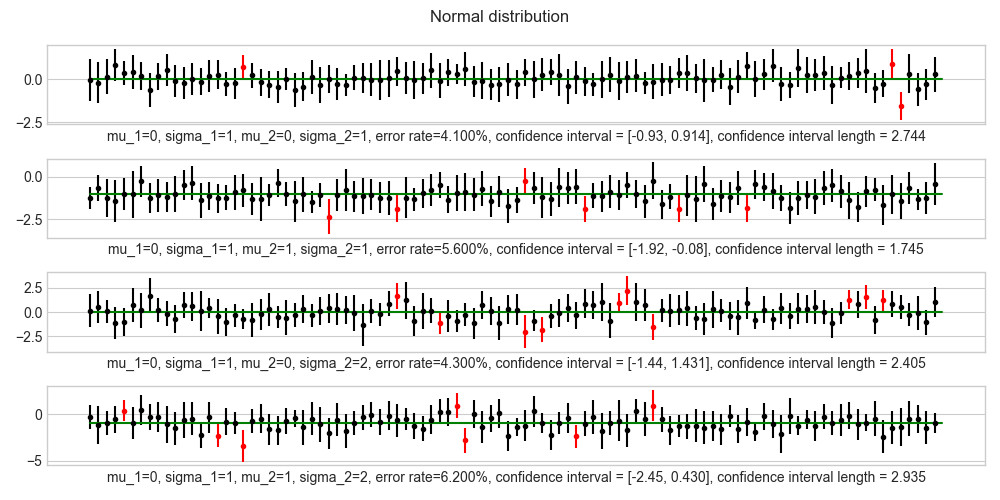
\includegraphics[scale=0.65]{Z6_a.png}

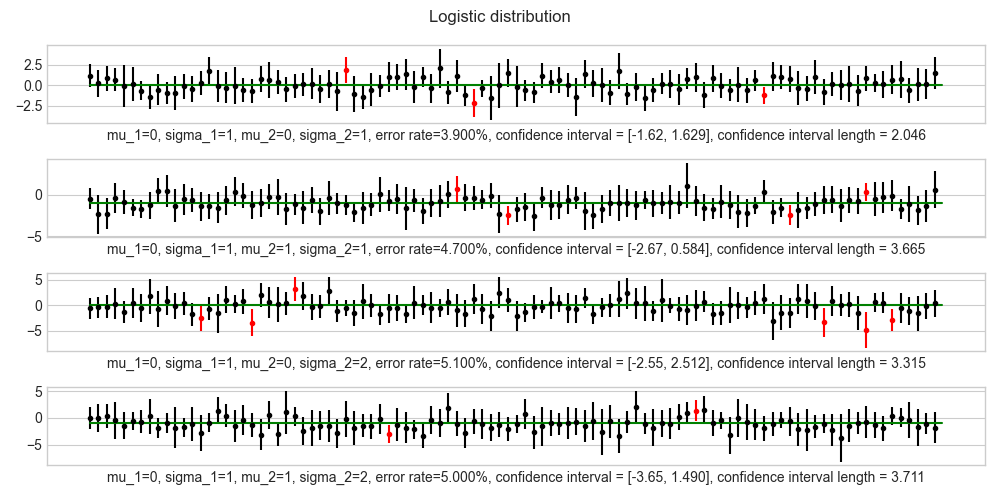
\includegraphics[scale=0.65]{Z6_b.png}

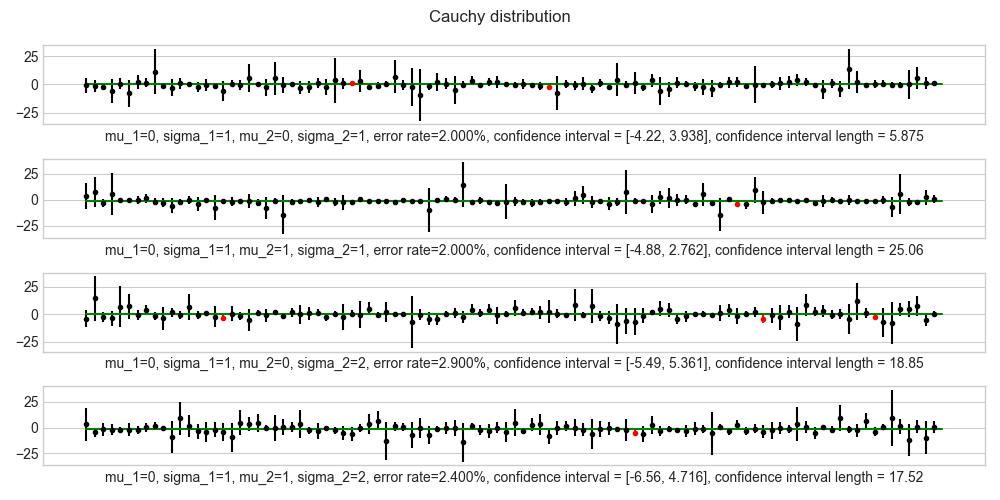
\includegraphics[scale=0.65]{Z6_c.png}

Znalezione przedziały ufności były znacznie dłuższe od tych wyznaczonych w zadaniu drugim. Mniejsza niepewność w zadaniu drugim prawdopodobnie wynika z dodatkowej wiedzy jaką jest wartość dokładna wariancji.

\section{Zadanie siódme}
Podaj przedział ufności dla ilorazu dwóch wariancji w modelu normalnym o znanych średnich na poziomie ufności $1-\alpha$. Uzasadnij jego postać.

\subsection{Rozwiązanie}
Tak samo jak w zadaniu dziewiątym, jednak korzystam ze znanych średnich do wyznaczenia estymatora wariancji.


\section{Zadanie ósme}
Powtórz eksperyment numeryczny z zadania 2 dla wybranych konfiguracji. Na jego podstawie oszacuj prawdopodobieństwo pokrycia nieznanego parametru przez przedział ufności z zadania 7 na poziomie ufności 0.95 oraz jego długość. Przedyskutuj uzyskane rezultaty.

\subsection{Rozwiązanie}

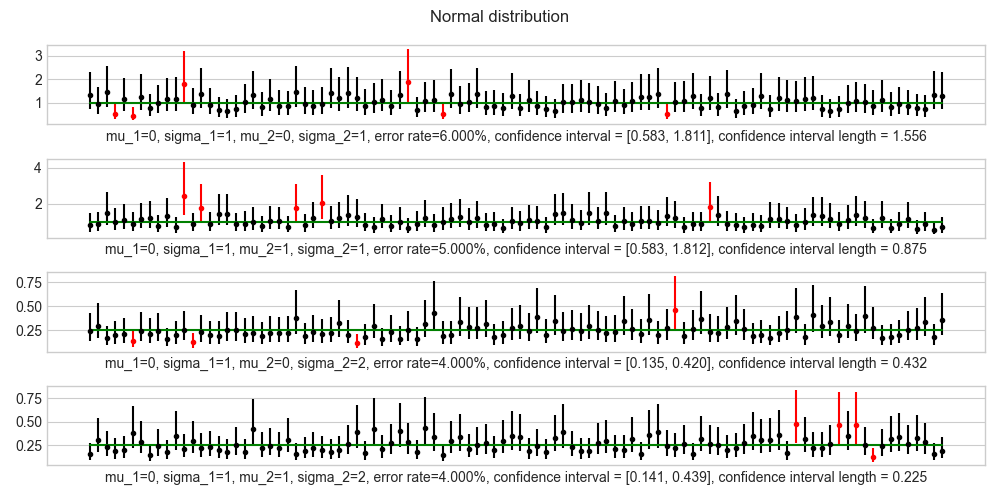
\includegraphics[scale=0.65]{Z8_a.png}

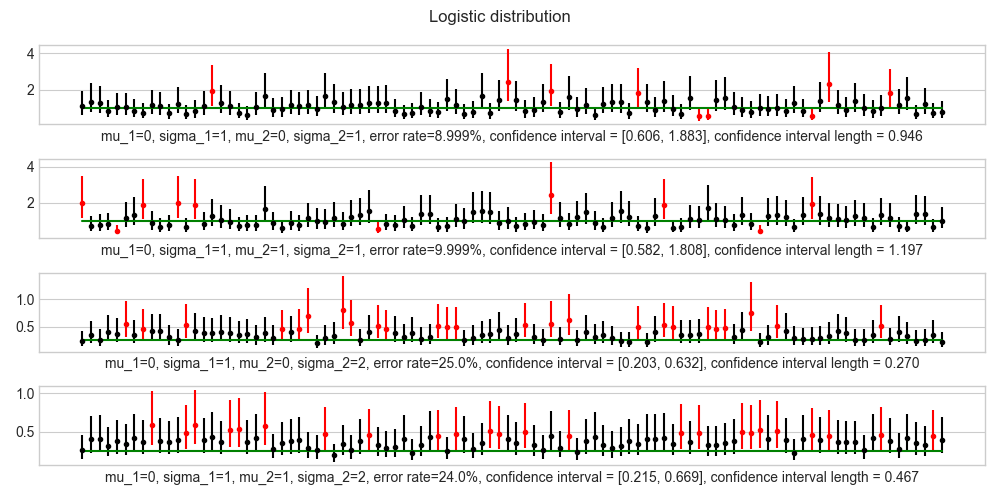
\includegraphics[scale=0.65]{Z8_b.png}

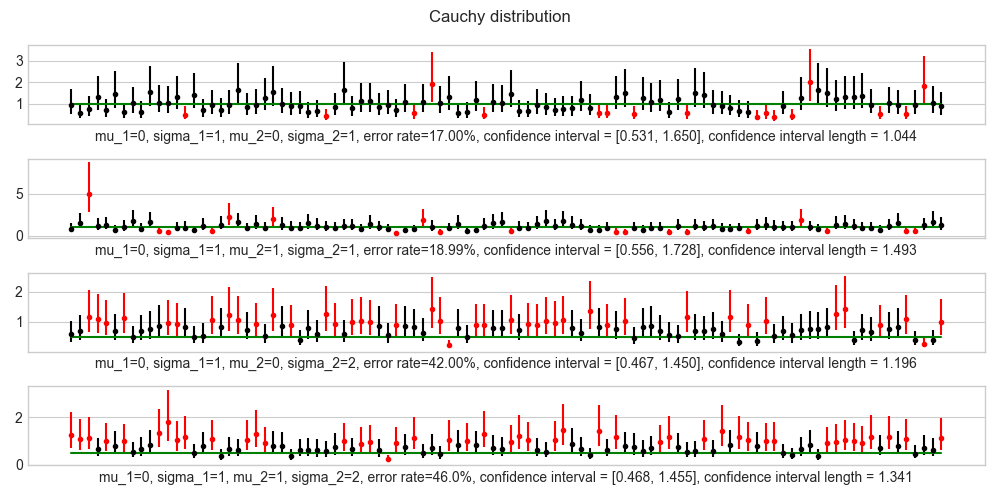
\includegraphics[scale=0.65]{Z8_c.png}


Rozkład Cauchy'ego stwarza duże problemy w zadaniu estymacji jego parametrów. Jak widać w wielu przypadkach przedziały ufności nie pokrywają faktycznej wartości. Może to wynikać z nie dość licznej próby.

\section{Zadanie dziewiąte}
Podaj przedział ufności dla ilorazu dwóch wariancji w modelu normalnym o nieznanych średnich na poziomie ufności $1-\alpha$. Uzasadnij jego postać.

\subsection{Rozwiązanie}
Estymatorem punktowym dla ilorazu $\frac{\sigma_1^2}{\sigma_2^2}$ jest $\frac{s_1^2}{s_2^2}$. Statystyka $\frac{s_1^2}{\sigma_1^2}/\frac{s_2^2}{\sigma_2^2}$ ma rozkład F z $n_1-1$ i $n_2-1$ stopniami swobody. Zatem:
$$P(F_{1-\alpha/2}<\frac{s_1^2}{\sigma_1^2}/\frac{s_2^2}{\sigma_2^2}<F_{\alpha/2})=1-\alpha$$
$$P(\frac{1}{F_{\alpha/2}}\frac{s_1^2}{s_2^2}<\frac{\sigma_1^2}{\sigma_2^2}<\frac{1}{F_{1-\alpha/2}}\frac{s_1^2}{s_2^2})=1-\alpha$$

Przedział ufności dla $\frac{\sigma_1^2}{\sigma_2^2}$ ma postać:
$$\left[\frac{1}{F_{\alpha/2}}\cdot\frac{s_1^2}{s_2^2},\frac{1}{F_{1-\alpha/2}}\cdot\frac{s_1^2}{s_2^2}\right]$$




\section{Zadanie dziesiąte}
Powtórz eksperyment numeryczny z zadania 2 dla wybranych konfiguracji. Na jego podstawie oszacuj prawdopodobieństwo pokrycia nieznanego parametru przez przedział ufności z zadania 9 na poziomie ufności 0.95 oraz jego długość. Przedyskutuj uzyskane rezultaty.


\subsection{Rozwiązanie}

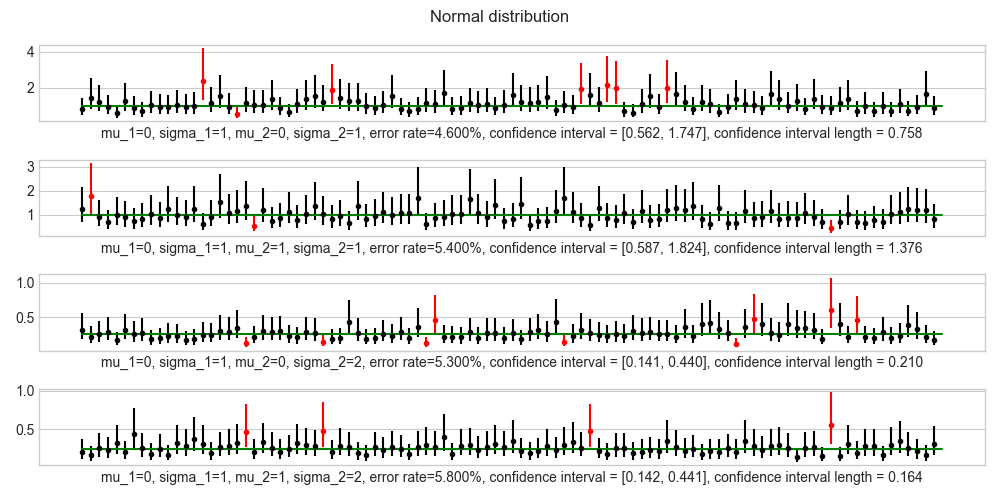
\includegraphics[scale=0.65]{Z10_a.png}

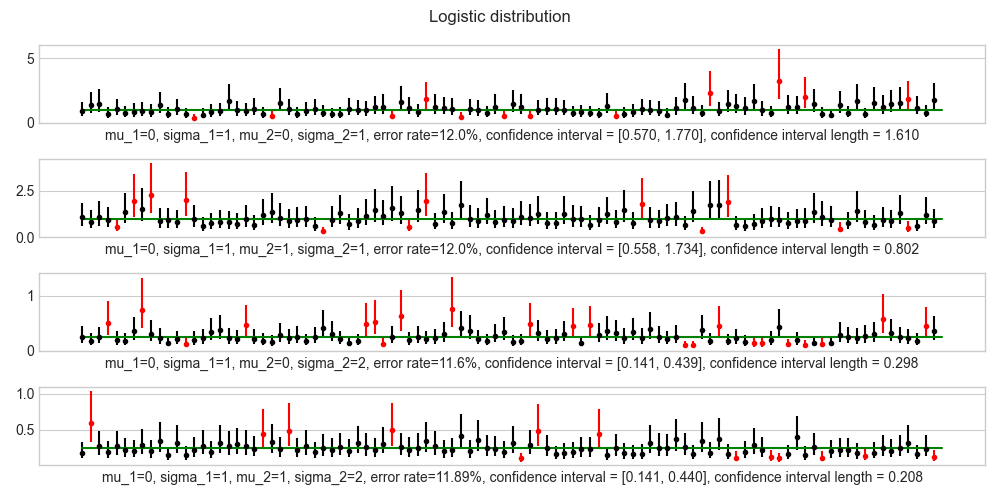
\includegraphics[scale=0.65]{Z10_b.png}

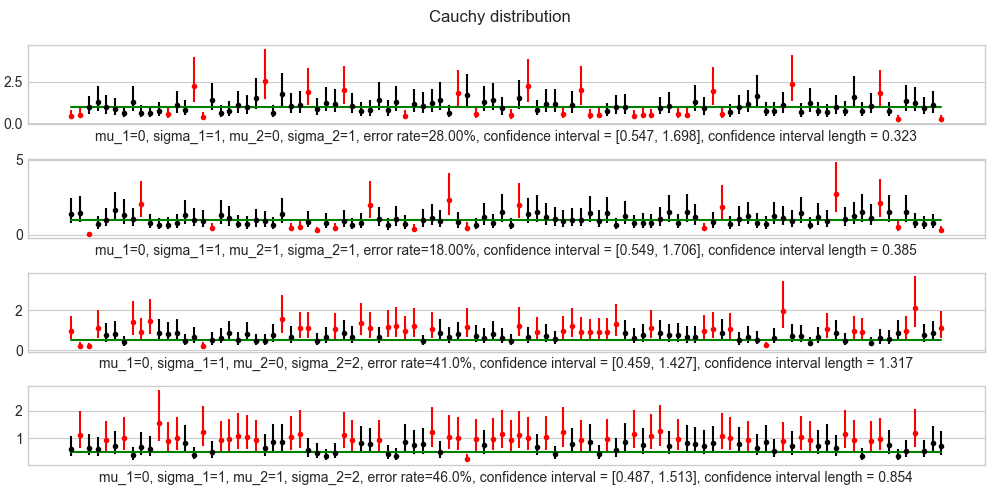
\includegraphics[scale=0.65]{Z10_c.png}


\section{Zadanie jedenaste}
Powtórz eksperyment numeryczny z zadań 2, 4, 6, 8, 10, dla $n_1=n_2=20$ i $n_1=n_2=100$. Przedyskutuj uzyskane rezultaty w nawiązaniu do wcześniejszych wyników.

\subsection{Rozwiązanie}

Dla przejrzystości nie będę zamieszczał wszystkich wykresów, opiszę jedynie główne obserwacje.
\begin{itemize}
\item Wraz ze wzrostem liczby obserwacji długość przedziału ufności maleje.
\item Eksperymenty dla $n=20$ cechują się znacznie większą zmiennością wyników.
\item Wartości error rate z zadania 2 faktycznie zmniejszają się wraz ze wzrostem liczebności próby.
\end{itemize}



\end{document}
